%%%%%%%%%%%%%%%%%%%%%%%%%%%%%%%%%%%%
% Slide options
%%%%%%%%%%%%%%%%%%%%%%%%%%%%%%%%%%%%

% Option 1: Slides with solutions

\documentclass[slidestop,compress,mathserif]{beamer}
\newcommand{\soln}[1]{\textit{#1}}
\newcommand{\solnGr}[1]{#1}

% Option 2: Handouts without solutions

% \documentclass[11pt,containsverbatim,handout]{beamer}
% \usepackage{pgfpages}
% \pgfpagesuselayout{resize to}[letterpaper,landscape,border shrink=5mm]
% \newcommand{\soln}[1]{ }
% \newcommand{\solnGr}{ }

%%%%%%%%%%%%%%%%%%%%%%%%%%%%%%%%%%%%
% Style
%%%%%%%%%%%%%%%%%%%%%%%%%%%%%%%%%%%%

\def\chpviii@path{../../Chp 8}
\def\chpix@path{../../Chp 9}
\input{../../lec_style.tex}

%%%%%%%%%%%%%%%%%%%%%%%%%%%%%%%%%%%%
% Preamble
%%%%%%%%%%%%%%%%%%%%%%%%%%%%%%%%%%%%

\title[Lecture 37]{MA213: Lecture 37}
\subtitle{Module 5: Linear regression}
\author{OpenIntro Statistics, 4th Edition}
\institute{$\:$ \\ {\footnotesize Based on slides developed by Mine \c{C}etinkaya-Rundel of OpenIntro. \\
The slides may be copied, edited, and/or shared via the \webLink{http://creativecommons.org/licenses/by-sa/3.0/us/}{CC BY-SA license.} \\
Some images may be included under fair use guidelines (educational purposes).}}
\date{}


%%%%%%%%%%%%%%%%%%%%%%%%%%%%%%%%%%%%
% Begin document
%%%%%%%%%%%%%%%%%%%%%%%%%%%%%%%%%%%%

\begin{document}


%%%%%%%%%%%%%%%%%%%%%%%%%%%%%%%%%%%%
% Title page
%%%%%%%%%%%%%%%%%%%%%%%%%%%%%%%%%%%%

{
\addtocounter{framenumber}{-1} 
{\removepagenumbers 
\usebackgroundtemplate{
\includegraphics[width=\paperwidth]{../../OpenIntro_Grid_4_3-01.jpg}}
\begin{frame}

\hfill 
\includegraphics[width=20mm]{../../oiLogo_highres}

\titlepage

\end{frame}
}
}


%%%%%%%%%%%%%%%%%%%%%%%%%%%%%%%%%%%%
% Recap/Agenda 
%%%%%%%%%%%%%%%%%%%%%%%%%%%%%%%%%%%%
% TODO better formatting
\begin{frame}
    \frametitle{Module 5: Linear regression}
    \begin{itemize}
        \item \hl{Previously: }Model Selection (Chapter 9.2)
        \item \hl{This time: }Checking model conditions using graphs (Chapter 9.3)
        \item \hl{Reading: }
        \item \hl{Deadlines/Announcements: }
    \end{itemize}
    
\end{frame}

%%%%%%%%%%%%%%%%%%%%%%%%%%%%%%%%%%%%
% Learning objectives:
%%%%%%%%%%%%%%%%%%%%%%%%%%%%%%%%%%%%
\begin{frame}
    \frametitle{Learning Objectives}
    \begin{itemize}
        \item \textbf{M5, LO3: Fit and Interpret Linear Models Using Least Squares:} Fit the intercept and slope of a linear model to data using the least squares method, interpret the fitted values, and use the model to predict responses to new inputs.
        \item \textbf{M5, LO4: Explain and Assess Model Fit:} Explain the least squares fitting procedure, assess whether the fit is unduly influenced by any particular points, and distinguish between interpolation and extrapolation in predictions.
        \item \textbf{M5, LO5: Perform Inference for Regression Coefficients:} Use fit summary and parameter estimates (e.g., $\hat{\beta}_1$ and $\hat{\sigma}^2$) to perform hypothesis tests or construct confidence intervals for the slope, and interpret the results.
    \end{itemize}
\end{frame}
    

%%%%%%%%%%%%%%%%%%%%%%%%%%%%%%%%%%%%
% Sections
%%%%%%%%%%%%%%%%%%%%%%%%%%%%%%%%%%%%

\begin{frame}
  \frametitle{Reminder: Simple Regression Model and Conditions}

We assume that the \textbf{residuals} are iid normally distributed:
\[y_i = \beta_0 + \beta_1 x_i + \epsilon_i \quad \text{ where } \epsilon_i \overset{\mathrm{iid}}{\sim} N(0, \sigma) \qquad i=1,2,\ldots,n \]

This is why we checked the conditions:
\begin{enumerate}

\item Linearity

\item Nearly normal residuals

\item Constant variability

\end{enumerate}

\end{frame}

%%%%%%%%%%%%%%%%%%%%%%%%%%%%%%%%%%%%

\begin{frame}
\frametitle{Residuals}

\hl{Residuals} are the leftovers from the model fit: [Data = Fit + Residual]

\begin{center}
\includegraphics[width=0.8\textwidth]{\chpviii@path/8-2_least_square_reg/figures/poverty/poverty_hsgrad_res}
\end{center}

\end{frame}

%%%%%%%%%%%%%%%%%%%%%%%%%%%%%%%%%%

\begin{frame}
\frametitle{Residuals (cont.)}

\formula{Residual}{
Residual is the difference between the observed ($y_i$) and predicted $\hat{y}_i$. 
\[ e_i = y_i - \hat{y}_i \]
}
\vspace{-0.5cm}
\twocol{0.6}{0.4}
{
\begin{center}
\includegraphics[width=\textwidth]{\chpviii@path/8-2_least_square_reg/figures/poverty/poverty_hsgrad_res_text}
\end{center}
}
{
% \pause
\begin{itemize}
\item \% living in poverty in DC is 5.44\% more than predicted.
% \pause
\item \% living in poverty in RI is 4.16\% less than predicted.
\end{itemize}
}
\end{frame}

%%%%%%%%%%%%%%%%%%%%%%%%%%%%%%%%%%%

\begin{frame}
\frametitle{An objective measure for finding the best line}

\begin{itemize}

\item We want a line that has small residuals:
% \pause
\begin{enumerate}
\item Option 1: Minimize the sum of magnitudes (absolute values) of residuals
\[ |e_1| + |e_2| + \cdots + |e_n| \]
% \pause
\item Option 2: Minimize the sum of squared residuals -- \hl{least squares}
\[ e_1^2 + e_2^2 + \cdots + e_n^2 \]
\end{enumerate}

\pause

\item Why least squares?
\pause
\begin{enumerate}
\item Most commonly used
% \pause
\item Easier to compute by hand and using software
% \pause
\item In many applications, a residual twice as large as another is usually more than twice as bad
% \pause
\item Has nice statistical properties under certain conditions...
\end{enumerate}

\end{itemize}

\end{frame}

%%%%%%%%%%%%%%%%%%%%%%%%%%%%%%%%%%

\begin{frame}
\frametitle{Slope and Intercept}

Estimate the slope and intercept by minimizing the sum of squared residuals -- \hl{least squares}
\[ \hat{\beta}_0, \hat{\beta}_1 = \underset{\beta_0,\beta_1}{argmin} \sum_{i=1}^{n} e_i^2 = \underset{\beta_0,\beta_1}{argmin} \sum_{i=1}^{n} |y_i-\hat{y}_i|^2 \]


\hl{Slope}
\[ b_1 = \frac{s_y}{s_x} R \]


\hl{Intercept}
\[ b_0 = \bar{y} - b_1 \bar{x} \]

\pause
\small{
\Note{The Least Squares solutions for $\beta_0$ and $\beta_1$ are the \hl{maximum likelihood estimators} for the intercept and slope if our Normal model is true. That means that they are the values of the parameters that assign the highest probability to the data that we observed. (More on this in later courses!)}
}

\end{frame}


%%%%%%%%%%%%%%%%%%%%%%%%%%%%%%%%%%

\begin{frame}
\frametitle{Conditions: (1) Linearity}

\begin{itemize}

\item The relationship between the explanatory and the response variable should be linear. 

% \pause

\item Methods for fitting a model to non-linear relationships exist, but are beyond the scope of this class. 

% \pause

\item Check using a scatterplot of the data, or a \hl{residuals plot}.

\end{itemize}

\begin{center}
\includegraphics[width=0.7\textwidth]{\chpviii@path/8-2_least_square_reg/figures/sampleLinesAndResPlots/sampleLinesAndResPlots}
\end{center}

\end{frame}

%%%%%%%%%%%%%%%%%%%%%%%%%%%%%%%%%%

\begin{frame}
\frametitle{Conditions: (2) Nearly normal residuals}

\begin{itemize}

\item The residuals should be nearly normal.

% \pause

\item This condition may not be satisfied when there are unusual observations that don't follow the trend of the rest of the data.

% \pause

\item Check using a histogram.

\end{itemize}

\begin{center}
\includegraphics[width=0.5\textwidth]{\chpviii@path/8-2_least_square_reg/figures/poverty/normal_res}
\end{center}

\end{frame}

%%%%%%%%%%%%%%%%%%%%%%%%%%%%%%%%%%

\begin{frame}
\frametitle{Conditions: (3) Constant variability}

\twocol{0.5}{0.5}
{
\begin{center}
\includegraphics[width=\textwidth]{\chpviii@path/8-2_least_square_reg/figures/poverty/poverty_hsgrad_tube}
\end{center}
}
{
\begin{itemize}

\item The variability of points around the least squares line should be roughly constant.

% \pause

\item This implies that the variability of residuals around the 0 line should be roughly constant as well.

% \pause

\item Also called \hl{homoscedasticity}.

% \pause

\item Check using a residuals plot.

\end{itemize}
}

\end{frame}
%%%%%%%%%%%%%%%%%%%%%%%%%%%%%%%%%%%%%%%%%%%%%%%%%%%%%%%%%%%%%%%%%%%%%%%%%%%%%%%%%%%%%%%%%%%%%%%%%%%%%%%%%%%%
% 9.3
%%%%%%%%%%%%%%%%%%%%%%%%%%%%%%%%%%%%%%%%%%%%%%%%%%%%%%%%%%%%%%%%%%%%%%%%%%%%%%%%%%%%%%%%%%%%%%%%%%%%%%%%%%%%

%%%%%%%%%%%%%%%%%%%%%%%%%%%%%%%%%%%%

\section{Multiple Regression: Checking model conditions using graphs}

%%%%%%%%%%%%%%%%%%%%%%%%%%%%%%%%%%%%

\subsection{Diagnostic plots}

%%%%%%%%%%%%%%%%%%%%%%%%%%%%%%%%%%%%

\begin{frame}
\frametitle{Multiple Linear Regression Model and Conditions}

\[ \hat{y} = \beta_0 + \beta_1 x_1 + \beta_2 x_2 + \cdots + \beta_p x_p \] 
\pause
Or:
\small{
\[y_i = \beta_0 + \beta_1 x_1 + \beta_2 x_2 + \cdots + \beta_p x_p + \epsilon_i \quad \]
\[\text{ where } \epsilon_i \overset{\mathrm{iid}}{\sim} N(0, \sigma) \qquad i=1,2,\ldots,n \]
}
\pause

The model depends on the following conditions
\begin{enumerate}
\item residuals are nearly normal (less important for larger data sets)\pause
\item residuals have constant variability\pause
\item residuals are independent\pause
\item each variable is linearly related to the outcome \pause \\
\end{enumerate}

We often use graphical methods to check the validity of these conditions

\end{frame}

%%%%%%%%%%%%%%%%%%%%%%%%%%%%%%%%%%

\begin{frame}
\frametitle{(1) nearly normal residuals}

normal probability plot and/or histogram of residuals: \\

\begin{center}
\includegraphics[width=0.6\textwidth]{\chpix@path/9-3_model_cond/figures/beauty/normal_res}
\end{center}

\dq{Does this condition appear to be satisfied?}

\end{frame}

\begin{frame}
\frametitle{How normal is normal enough?}
It depends on our goals:
\begin{itemize}
    \item If we are mainly interested in predicting the expected response for given predictor values, then minor deviations from normality are not a big concern
    \item If we are interested in precise inference for the regression coefficients (hypothesis tests, confidence intervals), then we want the residuals to be fairly normal
    \item If we are interested in predicting responses with \emph{prediction intervals}, then we want the residuals to be fairly normal
\end{itemize}
\pause
At least, we want to make sure there are no extreme deviations from normality (e.g., strong skewness, outliers).
\end{frame}

%%%%%%%%%%%%%%%%%%%%%%%%%%%%%%%%%%

\begin{frame}
\frametitle{(2) constant variability in residuals}

scatterplot of residuals and/or absolute value of residuals vs. fitted (predicted): \\

\begin{center}
\includegraphics[width=\textwidth]{\chpix@path/9-3_model_cond/figures/beauty/homo_res}
\end{center}

\dq{Does this condition appear to be satisfied?}

\end{frame}

%%%%%%%%%%%%%%%%%%%%%%%%%%%%%%%%%%

\begin{frame}
\frametitle{Checking constant variance - recap}

\begin{itemize}

\item When we did simple linear regression (one explanatory variable) we checked the constant variance condition using a plot of \hl{residuals vs. x}.

\item With multiple linear regression (2+ explanatory variables) we checked the constant variance condition using a plot of \hl{residuals vs. fitted}. 

\end{itemize}

$\:$ \\

\dq{Why are we using different plots?}

\soln{\only<2>{In multiple linear regression there are many explanatory variables, so a plot of residuals vs. one of them wouldn't give us the complete picture. (It's also smart to check the residuals vs. each explanatory variable individually to look for any patterns!)
}}

\end{frame}

%%%%%%%%%%%%%%%%%%%%%%%%%%%%%%%%%%

\begin{frame}[fragile]
\frametitle{(3) independent residuals}

scatterplot of residuals vs. order of data collection: \\

\begin{center}
\includegraphics[width=0.8\textwidth]{\chpix@path/9-3_model_cond/figures/beauty/indep_res}
\end{center}

\dq{Does this condition appear to be satisfied?}

\end{frame}

%%%%%%%%%%%%%%%%%%%%%%%%%%%%%%%%%%

\begin{frame}
\frametitle{More on the condition of independent residuals}

\begin{itemize}

\item Checking for independent residuals allows us to indirectly check for independent observations.

\item If observations and residuals are independent, we would not expect to see an increasing or decreasing trend in the scatterplot of residuals vs. order of data collection.

\item This condition is often violated when we have time series data. Such data require more advanced time series regression techniques for proper analysis.

\end{itemize}

\end{frame}

%%%%%%%%%%%%%%%%%%%%%%%%%%%%%%%%%%

\begin{frame}[fragile]
\frametitle{(4) linear relationships}

scatterplot of residuals vs. each (numerical) explanatory variable:

\begin{center}
\includegraphics[width=0.8\textwidth]{\chpix@path/9-3_model_cond/figures/beauty/linear}
\end{center}

\dq{Does this condition appear to be satisfied?}

\Note{We use residuals instead of the predictors on the y-axis so that we can still check for linearity without worrying about other possible violations like collinearity between the predictors.}

\end{frame}

%%%%%%%%%%%%%%%%%%%%%%%%%%%%%%%%

\section{R Demonstration: Checking model conditions using graphs}

%%%%%%%%%%%%%%%%%%%%%%%%%%%%%%%%%%%

\subsection{Options for improving the model fit}

%%%%%%%%%%%%%%%%%%%%%%%%%%%%%%%%%%%%

\begin{frame}
\frametitle{Several options for improving a model}

\begin{itemize}

\item Transforming variables
\item Seeking out additional variables to fill model gaps
\item Using more advanced methods that would account for challenges around inconsistent variability or nonlinear relationships between predictors and the outcome

\end{itemize}

\end{frame}

%%%%%%%%%%%%%%%%%%%%%%%%%%%%%%%%%%%%

\begin{frame}
\frametitle{Transformations}

If the concern with the model is non-linear relationships between the explanatory 
variable(s) and the response variable, transforming the response variable can be helpful. 

\begin{itemize}

\item Log transformation (log $y$)
\item Square root transformation ($\sqrt{y}$)
\item Inverse transformation ($1/y$)
\item Truncation (cap the max value possible)

\end{itemize}

It is also possible to apply transformations to the explanatory variable(s), however 
such transformations tend to make the model coefficients even harder to interpret.

\end{frame}

%%%%%%%%%%%%%%%%%%%%%%%%%%%%%%%%%%%%

\section{Edfinity Quiz: Transformations}

%%%%%%%%%%%%%%%%%%%%%%%%%%%%%%%%%%%%

\begin{frame}
\frametitle{Which transformation to use?}

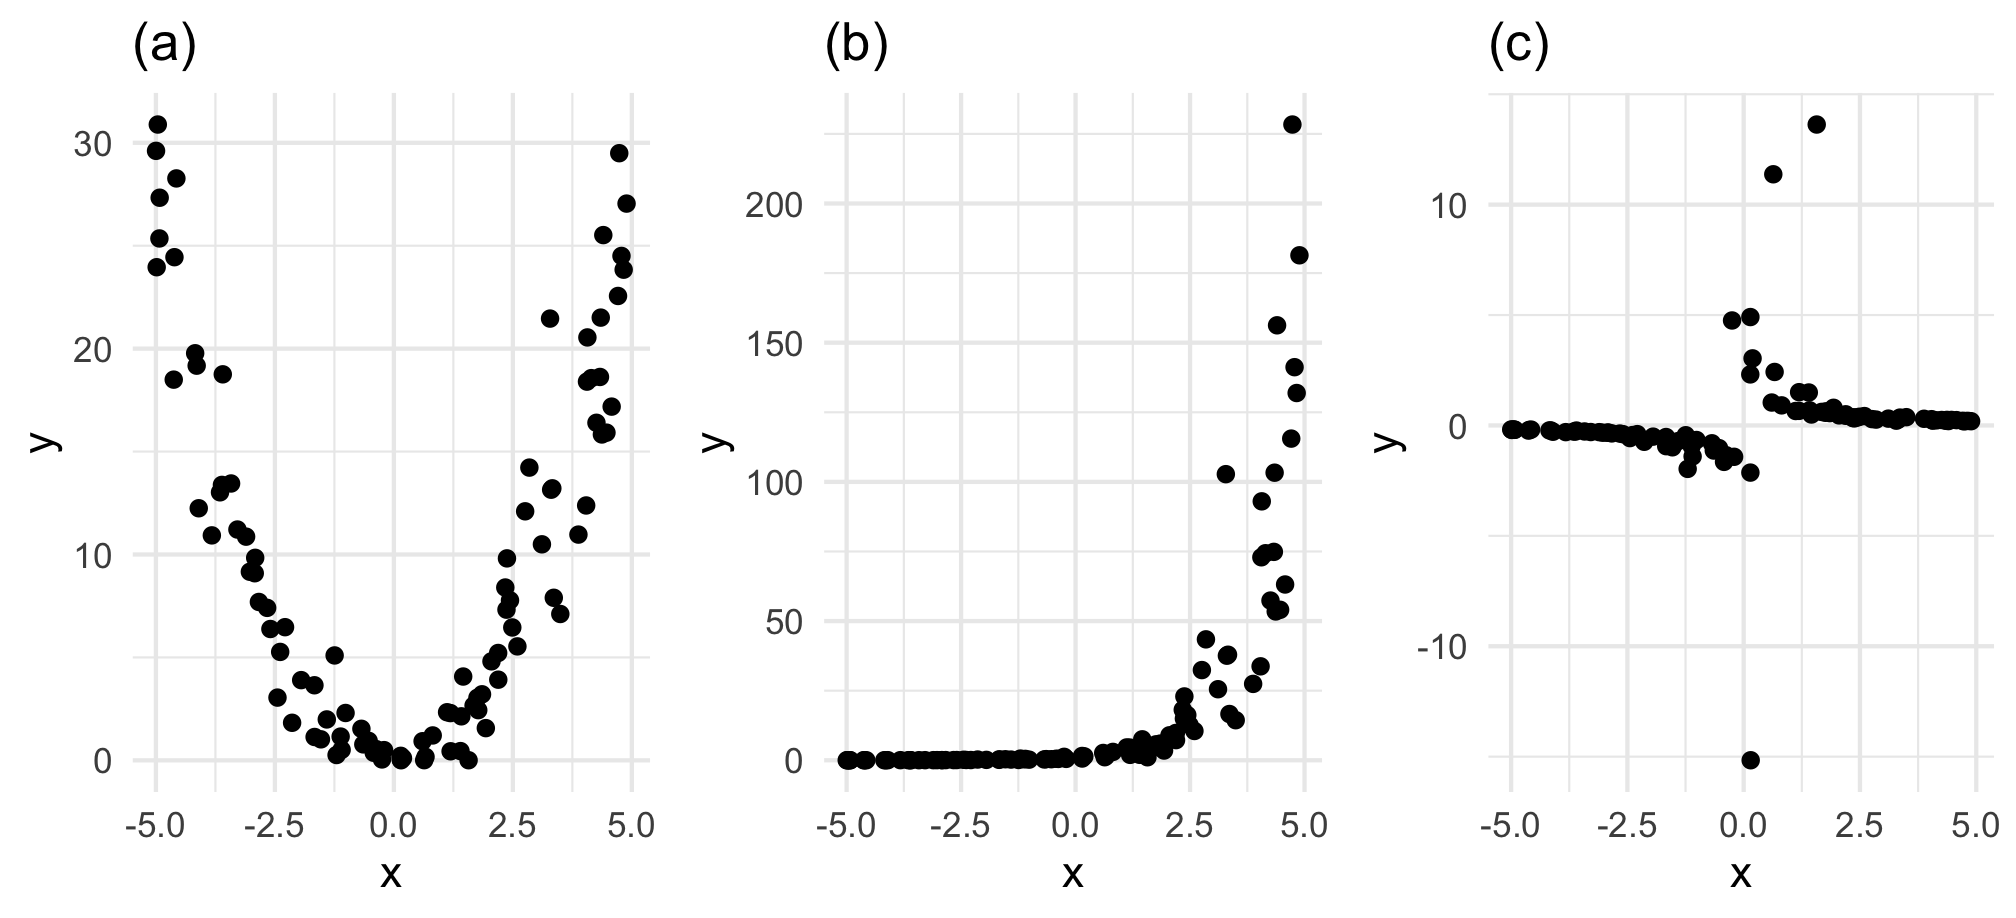
\includegraphics[height=0.4\textheight]{figures/transformations.png}

\soln{\only<2>{
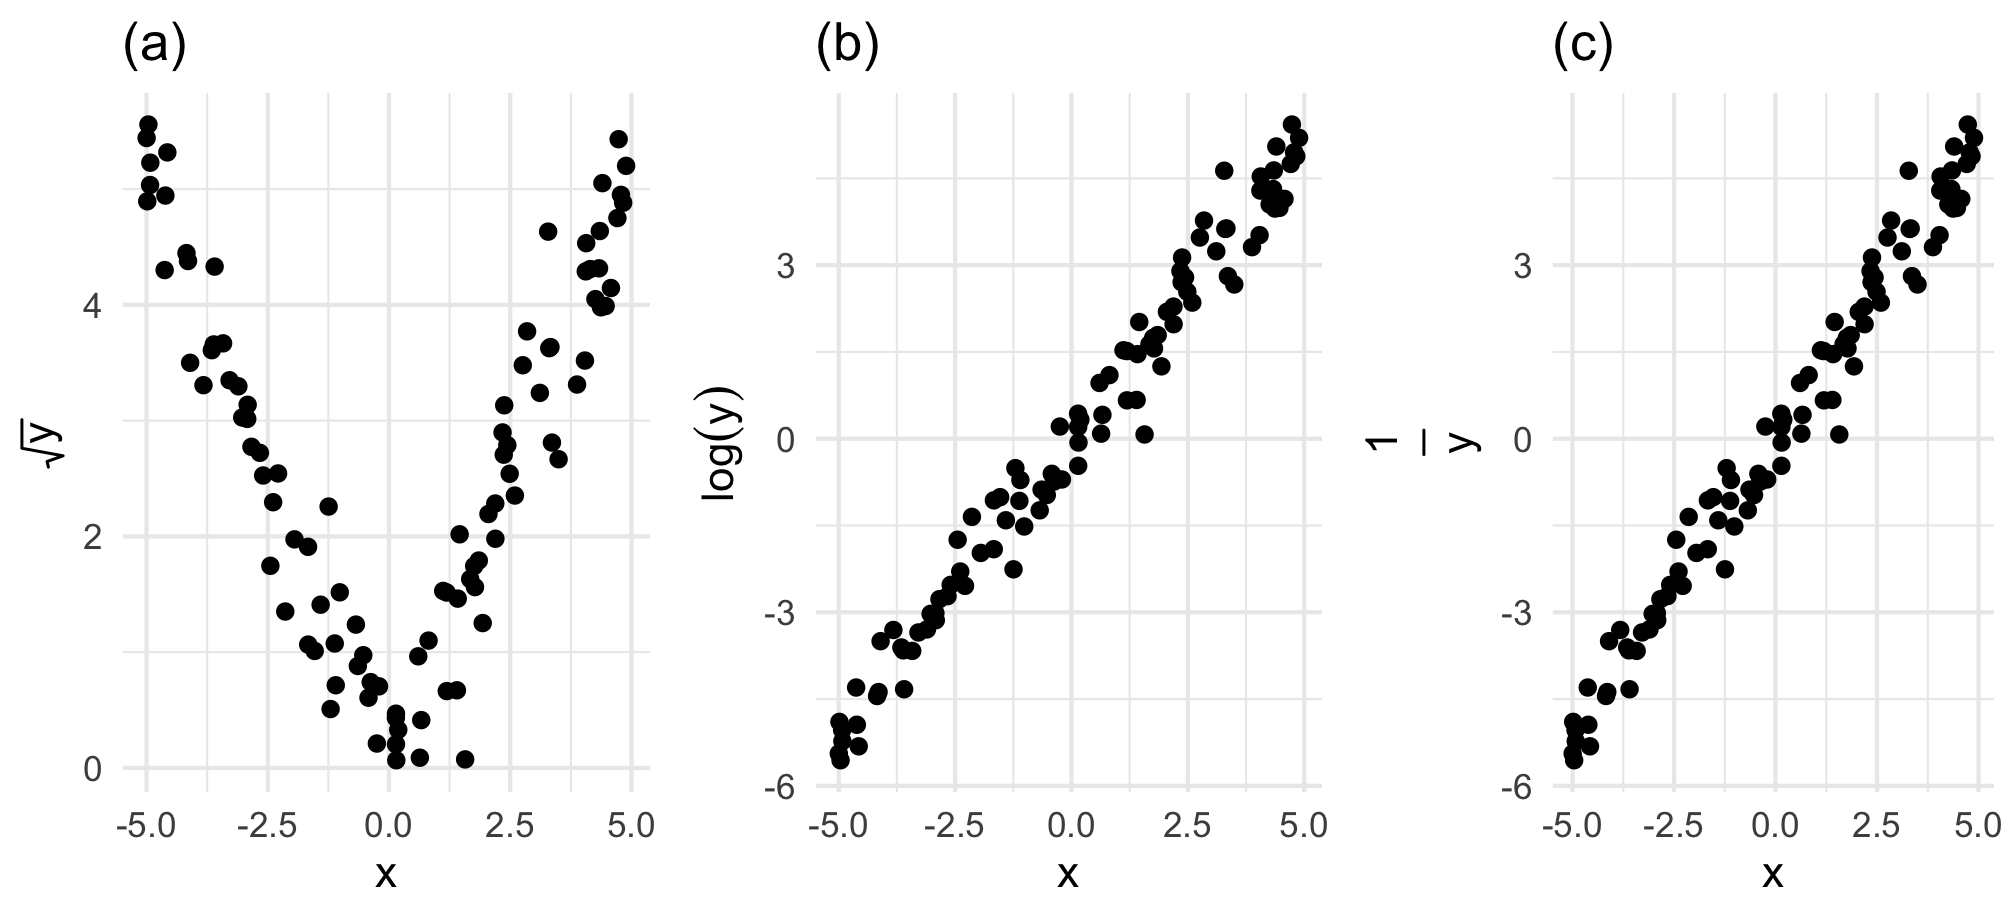
\includegraphics[height=0.4\textheight]{figures/transformations_applied.png}
}}

\end{frame}

%%%%%%%%%%%%%%%%%%%%%%%%%%%%%%%%%%%%

\begin{frame}
\frametitle{Models can be wrong, but useful}

\begin{quote}
All models are wrong, but some are useful. - George Box
\end{quote}

\begin{itemize}

\item No model is perfect, but even imperfect models can be useful, as long as we are clear and report the model's shortcomings.

\item If conditions are grossly violated, we should not report the model results, but instead consider a new model, even if it means learning more statistical methods or hiring someone who can help.

\end{itemize}

\end{frame}

%%%%%%%%%%%%%%%%%%%%%%%%%%%%%%%%%%%%


%%%%%%%%%%%%%%%%%%%%%%%%%%%%%%%%%%%%
% End document
%%%%%%%%%%%%%%%%%%%%%%%%%%%%%%%%%%%%

\end{document}